El modelo de producci\'on de Cobb--Douglas es
$$
P(T,K)=\beta_1 \, T^{\beta_2} \, K^{\beta_3},
$$
donde $P$ es la producci\'on total, $T$ es el trabajo, y $K$ es el capital. En este modelo el par\'ametro $\beta_1$ se interpreta como el factor total de productividad y los par\'ametros $\beta_2$ y $\beta_3$ como las elasticidades del trabajo y capital, respectivamente.

Descargue los datos disponibles en
\begin{center}
\url{https://goo.gl/aJJx4i}
\end{center}
este archivo contiene tres variables \texttt{P}, \texttt{T} y \texttt{K}, que representan respectivamente la producci\'on de salm\'on en Chile medida en toneladas, el sueldo promedio de un trabajador del salm\'on medido en miles de pesos y el PIB de esta industria medido en millones de d\'olares, durante los \'ultimos 12 meses.

En un rutero de \matlab llamado \texttt{cobbdouglas.m}
\begin{enumerate}
\item Cargue el archivo mencionado anteriormente.
\item Grafique en una misma ventana de figuras, usando \texttt{subplot}, los gr\'aficos de \texttt{P},\texttt{T} y \texttt{K} versus el mes en tras gr\'aficas distintas.
\item Calcule la producci\'on, sueldo y PIB promedio de la industria Salmonera durante los \'ultimos 12 meses.
\item A partir de los datos cargados ensamble y resuelva el sistema de ecuaciones lineales que permite calcular, por ajuste de m\'inimos cuadrados, los par\'ametros $\beta_1$, $\beta_2$ y $\beta_3$ de este modelo.

\textbf{Observaci\'on:} Antes de ensamblar las matrices del sistema debe linealizar este modelo. Para esto proponga una transformaci\'on del modelo en el siguiente casillero:

\respuesta{5cm}
\item Escriba a continuaci\'on los valores de los par\'ametros $\beta_1$, $\beta_2$ y $\beta_3$ calculados:

\respuesta{1cm}

\item Usando los par\'ametros calculados anteriormente, \textquestiondown Cu\'al ser\'ia la producci\'on si se tiene un PIB promedio pero se duplica el sueldo promedio de los trabajadores?.

\respuesta{1cm}
\end{enumerate}
\textbf{Desarrollo:} 
\begin{enumerate}
\item[a-b)] El programa debe tener instrucciones similares a
\begin{lstlisting}
clear all; close all; clc;
load salmones.mat
subplot(1,3,1);plot(K);
subplot(1,3,2);plot(T);
subplot(1,3,3);plot(P);
\end{lstlisting}
con las cuales se debe hacer un gr\'afico como
\begin{center}
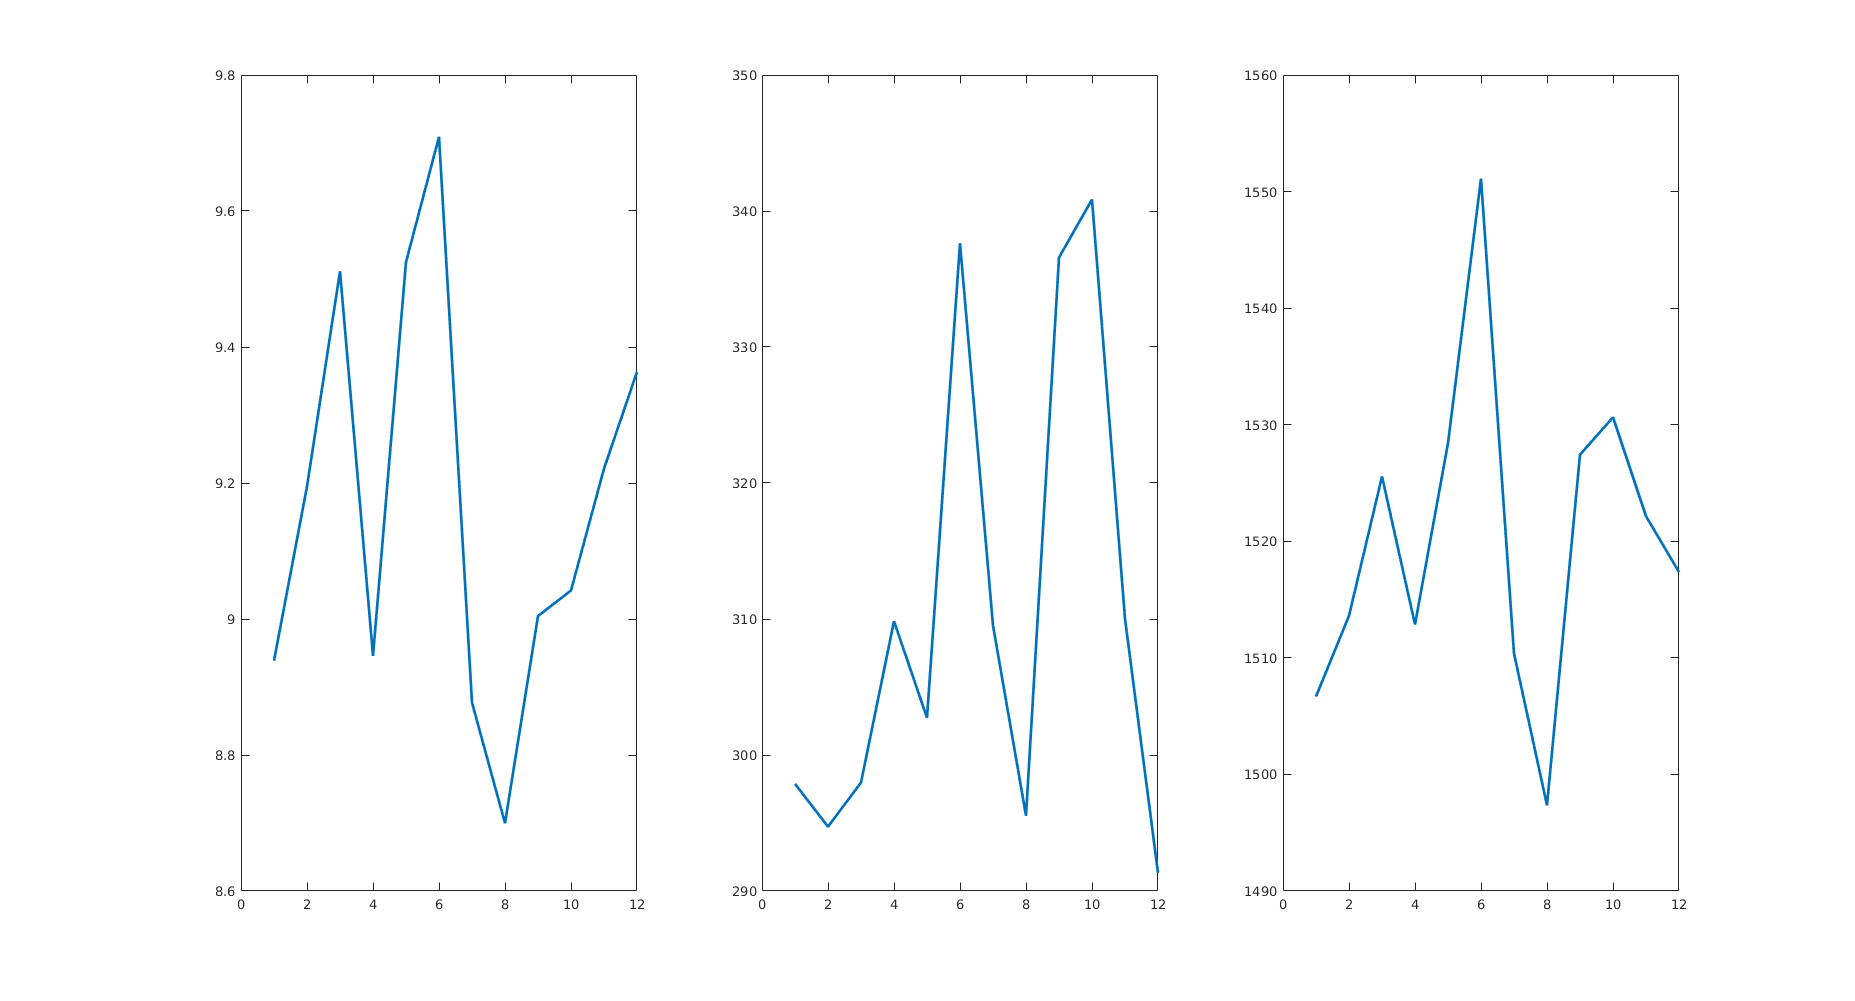
\includegraphics[width=0.8\textwidth]{./cobb-douglas.png}
\end{center}

\item[c)] El modelo se linealiza mediante la funci\'on logaritmo natural, seg\'un
$$
ln(P)=ln(\beta_1)+\beta_2\,ln(T)+\beta_3\,ln(K)
$$
de donde se ensambla un sistema matricial similar a
\begin{lstlisting}
>> A=[ones(size(K))',log(T)',log(K)'];
b=log(P)';
coef=A\b

coef =

    6.3099
    0.1000
    0.2000
\end{lstlisting}
\item[d)] De lo anterior sigue que
$$
\beta_1=e^{{6.3099}}=550, \quad \beta_2=0.1,\quad \beta_3=0.2
$$

\item[e)] En el rutero se calculas los promedios de los datos descargados, seg\'un
\begin{lstlisting}
>> kmean=mean(K)
tmean=mean(T)
pmean=mean(P)

kmean =

    9.1693


tmean =

  310.3846


pmean =

   1.5203e+03
\end{lstlisting}
\item Usando los datos anteriores
\begin{lstlisting}
>> nuevaProduccion=exp(coef(1))*(2*tmean)^coef(2)*tmean^coef(3)

nuevaProduccion =

   3.2964e+03
\end{lstlisting}
as\'i en este escenario se producir\'an 3.296 toneladas de salm\'on.
\end{enumerate}



